Este capítulo apresentará o método proposto por este trabalho para o projeto de uma prótese ativa baseada em sensores e aprendizado de máquina.

\section{Visão geral do método}
\label{sec:metodo_protese}

O projeto desenvolvido neste trabalho é uma prótese robótica para membros inferiores ou, mais especificamente, para a articulação do tornozelo. Esta prótese será construída a partir de modelos de próteses para impressoras 3D, aproveitando-se as partes mecânicas. A intenção é manter um baixo custo de produção. O sistema é projetado para funcionar em uma prótese transtibial, atuando sobre ela para adaptar a rigidez da articulação conforme a situação.

\begin{figure}[h]
	\caption{\label{fig:big_picture}Visão geral do protótipo}
	\begin{center}
	    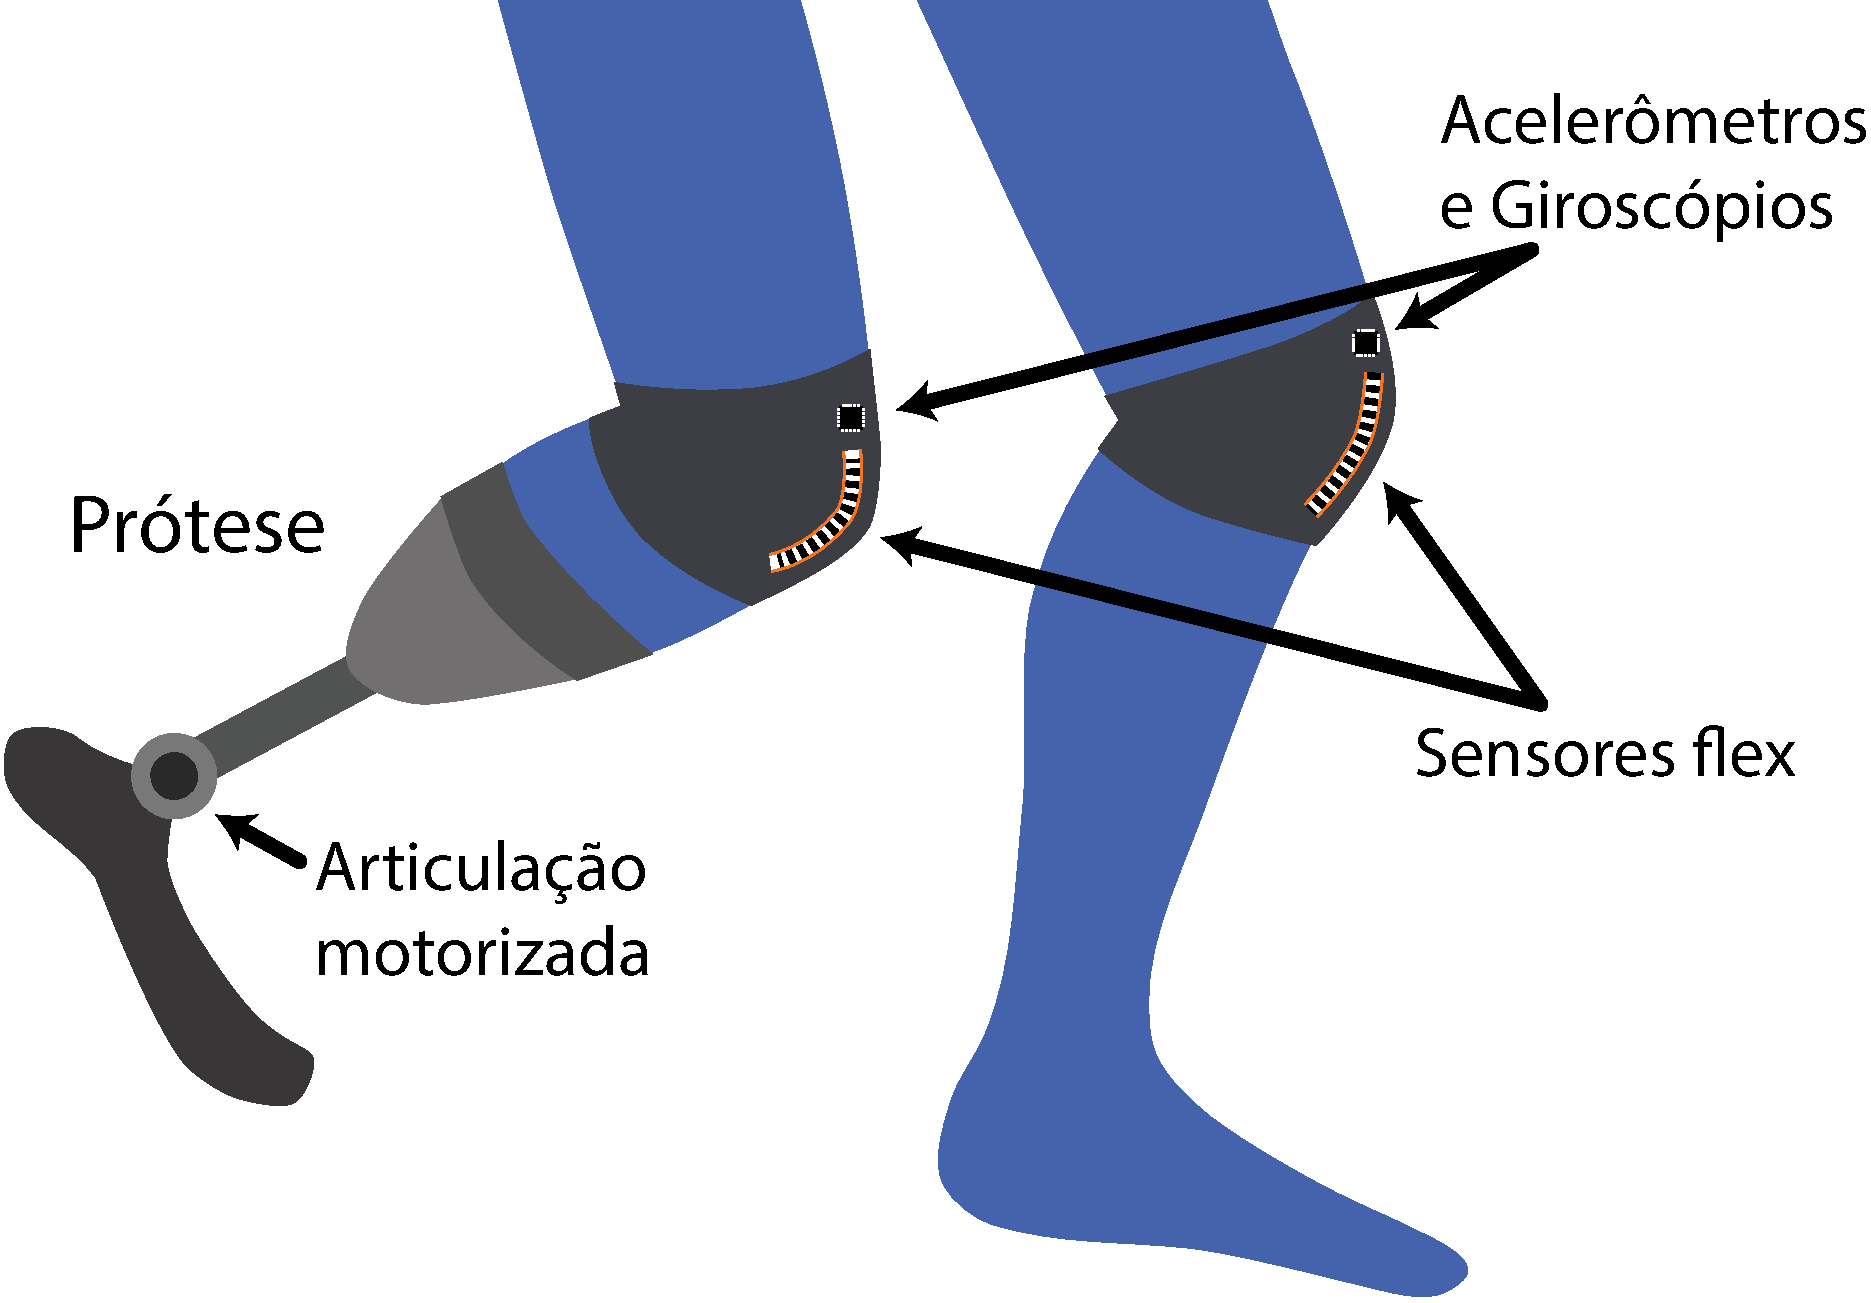
\includegraphics[width=0.6\textwidth]{resources/big_picture}
	\end{center}
	\legend{Fonte: Elaborada pelo autor}
\end{figure}

O sistema computacional que envolve o projeto estará equipado com sensores flex nas articulações dos joelhos além de giroscópios e acelerômetros, que serão usados para capturar as ações do usuário. A figura~\ref{fig:big_picture} ilustra a visão geral do sistema, incluindo o posicionamento dos sensores e o atuador da prótese em si.

Os sensores serão posicionados nos joelhos do usuário, e os dados capturados serão transmitidos a uma placa de processamento, que se comunicará com o atuador, de forma a adaptar a pisada do usuário de acordo com o ambiente. Conforme mostra a figura~\ref{fig:flowchart}, a prótese terá diferentes ajustes dependendo do tipo de ação, seja em caminhadas em planos, subida ou descida de escadas.

\todo{Terminar o fluxograma}\begin{figure}[h]
	\caption{\label{fig:flowchart}Fluxograma de funcionamento da prótese}
	\begin{center}
	    \includegraphics[width=\textwidth]{resources/flowchart}
	\end{center}
	\legend{Fonte: Elaborada pelo autor}
\end{figure}

\section{Prototipação da prótese}
\todo[inline,color=lightgray]{Descrever o funcionamento da prótese via algum modelo}
\subsection{Arquitetura do software}
\todo[inline,color=lightgray]{Diagrama UML}
\subsection{Arquitetura do hardware}
\todo[inline,color=lightgray]{Descrever os componentes da prótese: o motor, como funciona o motor e tal}

\section{Coleta de dados}
\todo[inline,color=lightgray]{Descrever que dados serão coletados (de que sensores) e como serão coletados, armazenados, etc.}

\section{Previsão de movimentos}
Os dados coletados serão analisados por um algoritmo de aprendizado de máquina para que se classifique e se preveja as ações do usuário. Essas ações serão classificadas de acordo com o passo a ser dado, podendo ser caminhada plana, subida ou descida de degrau.

Antes que o usuário realize um passo, o sistema deverá identificar em que ambiente este passo será dado. Isto poderá ser feito a partir do passo anterior, realizado pela perna intacta, e a partir do movimento atual extraído do membro residual.

Considerando que teremos um conjunto predeterminado de cenários possíveis -- caminhada plana, subida e descida de escada -- será decidida uma técnica de aprendizado de máquina supervisionado, mais especificamente de classificação, através de ferramentas de aprendizado de máquina, como as descritas na seção~\ref{sec:ml_tools}.

Assim que um passo começa a ser realizado, são acionados os atuadores, que terão sua ação determinada de acordo com o ambiente identificado, facilitando assim a locomoção do usuário.\todo{Não consigo identificar exatamente a dificuldade a ser resolvida em cada cenário para determinar \textbf{o que o motor deve fazer} especificamente.}

\section{Diagnóstico do uso da prótese e recomendações de melhorias no caminhar}
Os dados dos sensores também serão automaticamente armazenados para geração de estatísticas que podem ser usadas para diagnóstico relacionado à saúde da caminhada do usuário. O sistema fará um relatório do uso, indicando se é exercida mais força em uma das pernas do que na outra, por exemplo, além de outros dados.

A partir das informações geradas, poderá ser feitas recomendações de melhorias ao indivíduo, para que se melhore a postura, a caminhada, ou que se utilize algum tipo de equipamento adicional. Além disso, ainda será possível analisar as estatísticas de uso da prótese para avaliar seu impacto na vida do usuário, caso esteja alterando seus hábitos de alguma forma.

Para que este diagnóstico seja possível, será analisada a hipótese do uso de sensores adicionais aos propostos pelo protótipo atual, caso estes não sejam suficientes para gerar os dados necessários de análise de saúde da caminhada.